\documentclass{acm_sen_article}


\usepackage{color}
% correct bad hyphenation here
\hyphenation{op-tical net-works semi-conduc-tor}
%\renewcommand{\baselinestretch}{0.93}

\begin{document}
%
% paper title
% Titles are generally capitalized except for words such as a, an, and, as,
% at, but, by, for, in, nor, of, on, or, the, to and up, which are usually
% not capitalized unless they are the first or last word of the title.
% Linebreaks \\ can be used within to get better formatting as desired.
% Do not put math or special symbols in the title.
\title{SMT-Based Context-Bounded Model Checking for Embedded Systems: Challenges and Future Trends}


% author names and affiliations
% use a multiple column layout for up to three different
% affiliations
\author{Lucas C. Cordeiro \\
Electronic and Information Research Center\\
Federal University of Amazonas, Brazil\\
Email: lucascordeiro@ufam.edu.br
\and
Eddie B. de Lima Filho \\
Science, Technology, and Innovation Center\\ for the Industrial Pole of Manaus, Brazil \\
Email: eddie@ctpim.org.br}
%\IEEEauthorblockN{Homer Simpson}
%\IEEEauthorblockA{Twentieth Century Fox\\
%Springfield, USA\\
%Email: homer@thesimpsons.com}
%\and
%\IEEEauthorblockN{James Kirk\\ and Montgomery Scott}
%\IEEEauthorblockA{Starfleet Academy\\
%San Francisco, California 96678--2391\\
%Telephone: (800) 555--1212\\
%Fax: (888) 555--1212}}

% conference papers do not typically use \thanks and this command
% is locked out in conference mode. If really needed, such as for
% the acknowledgment of grants, issue a \IEEEoverridecommandlockouts
% after \documentclass

% for over three affiliations, or if they all won't fit within the width
% of the page, use this alternative format:
% 
%\author{\IEEEauthorblockN{Michael Shell\IEEEauthorrefmark{1},
%Homer Simpson\IEEEauthorrefmark{2},
%James Kirk\IEEEauthorrefmark{3}, 
%Montgomery Scott\IEEEauthorrefmark{3} and
%Eldon Tyrell\IEEEauthorrefmark{4}}
%\IEEEauthorblockA{\IEEEauthorrefmark{1}School of Electrical and Computer Engineering\\
%Georgia Institute of Technology,
%Atlanta, Georgia 30332--0250\\ Email: see http://www.michaelshell.org/contact.html}
%\IEEEauthorblockA{\IEEEauthorrefmark{2}Twentieth Century Fox, Springfield, USA\\
%Email: homer@thesimpsons.com}
%\IEEEauthorblockA{\IEEEauthorrefmark{3}Starfleet Academy, San Francisco, California 96678-2391\\
%Telephone: (800) 555--1212, Fax: (888) 555--1212}
%\IEEEauthorblockA{\IEEEauthorrefmark{4}Tyrell Inc., 123 Replicant Street, Los Angeles, California 90210--4321}}



% make the title area
\maketitle

% As a general rule, do not put math, special symbols or citations
% in the abstract
\begin{abstract}
The dependency on the correct functioning of embedded systems is rapidly growing, mainly due to their wide range of applications, such as micro-grids, automotive device control ({\it e.g.}, airbag control), health care, surveillance, mobile devices, and consumer electronics. Their structures are becoming more and more complex and now require multi-core processors with scalable shared memory, in order to meet increasing computational power demands. As a consequence, reliability of embedded (distributed) software becomes a key issue during system development, which must be carefully addressed and assured. Normally, state-of-the-art verification methodologies for embedded systems generate test vectors (with constraints) and use assertion-based verification and high-level processor models, during simulation; however, other additional challenges have been raised: the need for meeting time and energy constraints, handling concurrent software, dealing with platform restrictions, evaluating implementation-structure choices, and supporting legacy designs (usually written in low-level languages). The present paper discusses challenges, problems, and recent advances to ensure correctness and timeliness regarding embedded systems. Reliability issues, in the development of micro-grids and cyber-physical systems, are then considered, as a prominent (bounded) model checking application.
\end{abstract}

%\IEEEpeerreviewmaketitle


%--------------------------------------
\section{Introduction}
%--------------------------------------

Generally, embedded computer systems perform dedicated functions with high degree of reliability. They are used in a variety of sophisticated applications, which range from entertainment software, such as games and graphics animation, to safety-critical systems, such as nuclear reactors and automotive controllers~\cite{Kopetz11}. Embedded systems are ubiquitous, in modern day information systems, and are also becoming increasingly important in our society, especially in micro-grids, where reliability and carbon emission reduction are of paramount importance~\cite{xu15}, and in cyber-physical systems (CPS), which demand short development cycles and again a high-level of reliability~\cite{leeCPS,leeCPS2}. As a consequence, human life has also become more and more dependent on the services provided by this type of system and, in particular, their success is strictly related to both service relevance and quality. 

Figure~\ref{intelligent-product} shows some examples of embedded systems, which typically consist of a human-machine interface ({\it e.g.}, keyboard and LCD) and an instrumentation interface ({\it e.g.}, sensor, network, and actuator). Indeed, many current embedded systems, such as unmanned aerial vehicles (UAVs)~\cite{groza2015formal} and medical monitoring systems~\cite{Cordeiro09}, become interesting solutions only if they can reliably perform their target tasks. For instance, UAVs are a trend on military missions due to the absence of pilots; however, an incorrect plan execution may also cost human lives, which is unacceptable. In addition, wrong disease diagnosis or condition-evaluation reports have the potential to compromise patients' health with serious consequences.
%
\begin{figure}[!t]
	\centering
	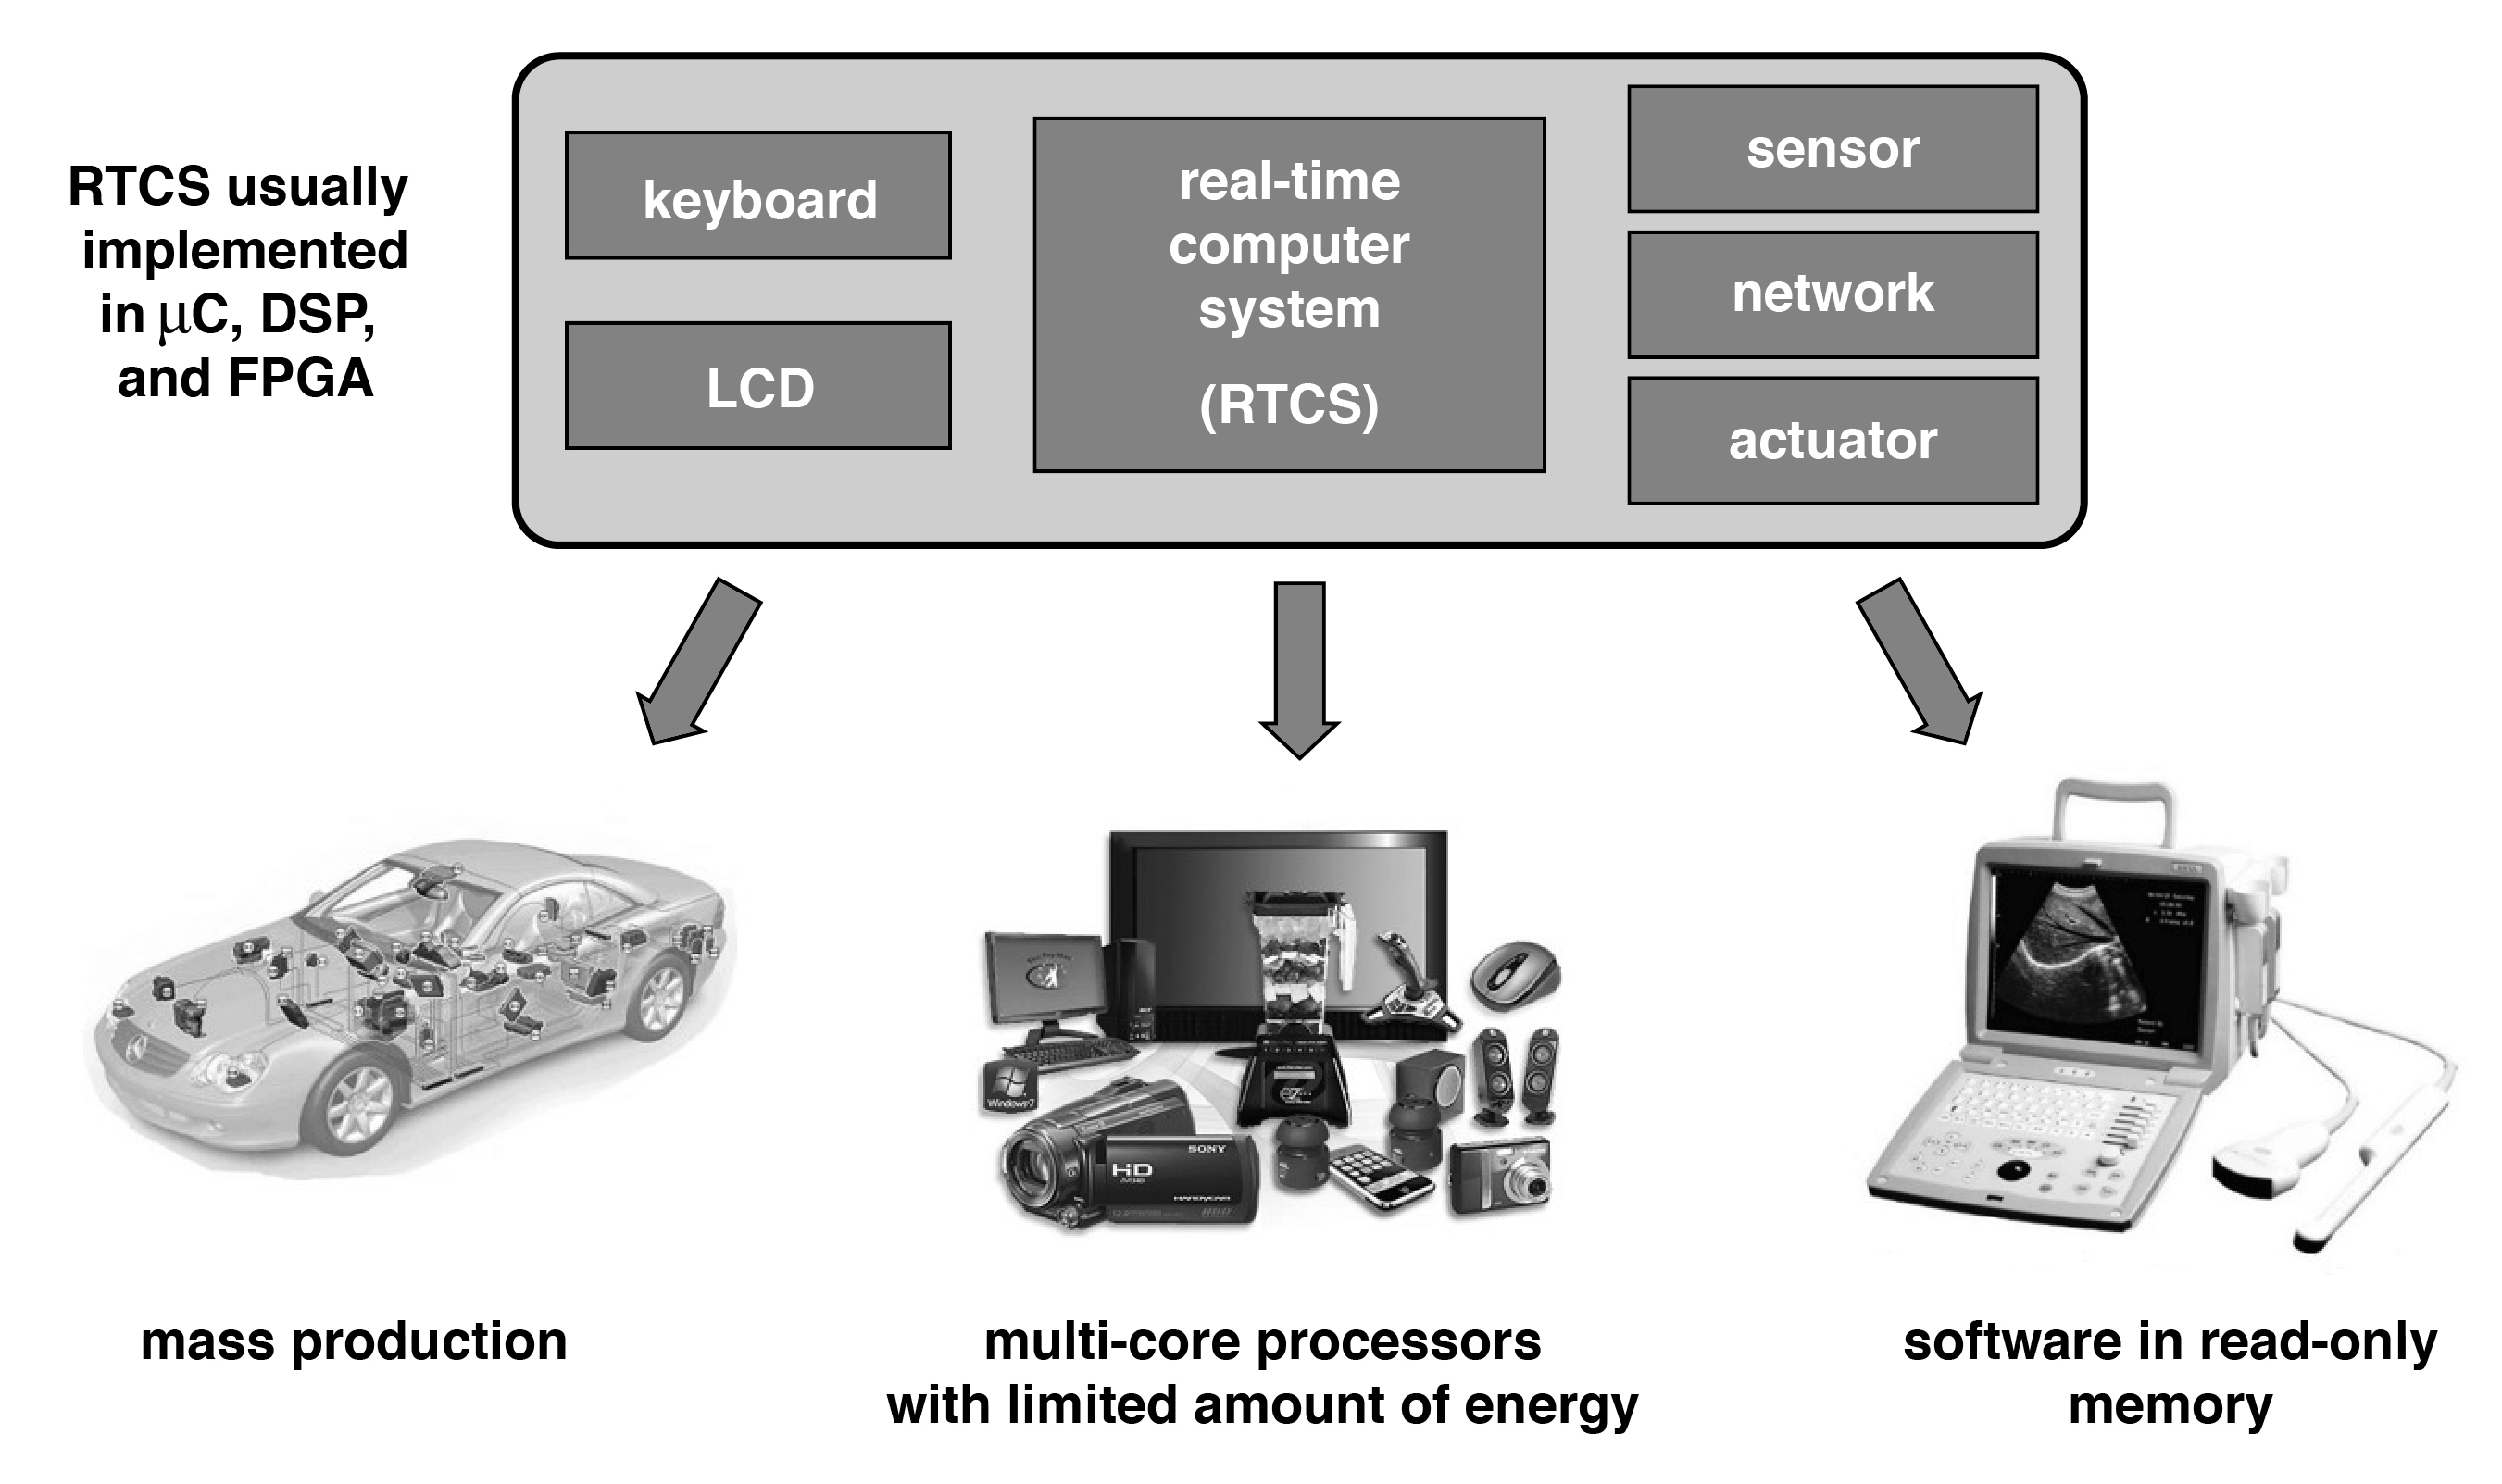
\includegraphics[scale=0.35]{figure1.eps}
	\caption{Embedded system is part of a well-specified larger system (intelligent product).}
	\label{intelligent-product}
\end{figure}

Besides, when physical interaction with the real world is needed, which happens in CPS, additional care must be taken, mainly when human action is directly replaced, as in vehicle driving. Regarding the latter, even human-in-the-loop feedback control can be employed \cite{munir}, which then raises deeper concerns related to the reliability of human behavior modeling and system implementation. Consequently, it is important to go beyond design correctness and also address behavior correctness, which may be performed by incorporating system models.

A number of distinctive characteristics might influence the embedded system development and verification process, which include: mass production and static structure, functionality determined by software in read-only memory, multi-core processors with scalable shared memory, and limited amount of energy. Additionally, the increasing computational power and decreasing size and cost, which are common to the area of computer processors, are enabling system designers to move more features to software domain, which consequently leads to difficulties in verifying design correctness, since stringent constraints imposed by the underlying hardware ({\it e.g.}, real-time, memory allocation, interrupts, and concurrency) must be considered during verification~\cite{Kroening15}.


%--------------------------------------
\section{Bounded Model Checking (BMC)}
%--------------------------------------

Bounded Model Checking (BMC) based on Boolean Satisfiability (SAT) was originally proposed to verify hardware designs~\cite{Biere99,handbook09}. The authors were able to successfully verify large digital circuits with approximately $9510$ latches and $9499$ inputs, leading to BMC formulae with $4 \times 10^6$ variables and $1.2 \times 10^7$ clauses to be checked by a standard SAT solver. BMC based on Satisfiability Modulo Theories (SMT)~\cite{BarrettSST09} was originally proposed to deal with increasing software verification complexity~\cite{Armando06}. 

In general, BMC techniques aim to check the violation of a given (safety) property at a given system's depth, {\it i.e.}, given a transition system \textit{M}, which is derived from the control-flow graph of a program; a property $\phi$ that represents the program correctness and/or the system's behaviour; and a bound of iterations \textit{k}, which limits the loop unrolling, data structures, and context-switches, BMC techniques thus unfold the system \textit{k} times, in order to convert it into a verification condition $\psi$, expressed in propositional logic or in a decidable-fragment of first-order logic, such that $\psi$ is \textit{satisfiable} if and only if $\phi$ has a counterexample of depth less than or equal to \textit{k}.

From the practical point of view, SAT-based or SMT-based BMC procedures have been successfully applied to verify a large number of hardware and software systems, including digital circuits, single- and multi-threaded programs. Those BMC techniques were able to find subtle bugs in real digital and embedded software systems, as reported in the literature~\cite{Clarke04,MerzFS12,CordeiroF11,Ivancic05,Cordeiro12}. However, the main criticism with respect to BMC techniques relies on completeness since they are able to prove system correctness only if an upper bound \textit{k} is known, {\it i.e.}, a bound that unfolds all loops and recursive functions to their maximum possible depth. 

Due to that limitation, BMC tools are typically susceptible to exhaustion of time or memory limits, when checking complex circuits implementation or programs with loops whose bounds are too large or cannot be statically determined.  

%In order to reason about embedded software accurately, an SMT-based BMC must consider a number of issues that are not easily mapped into the (background) theories supported by SMT solvers, {\it e.g.}, real-time, memory allocation, interrupts, and concurrency. Moreover, BMC techniques are able to falsify properties up to a depth \textit{k}. Consequently, they are able to prove system correctness only if an upper bound \textit{k} is known, {\it i.e.}, a bound that unfolds all loops and recursive functions to their maximum possible depth. In particular, BMC techniques limit the addressed regions of data structures ({\it e.g.}, arrays) and the number of loop iterations to a given bound $k$, which then restricts the state space that must be explored during verification, in such a way that real errors in applications \cite{Clarke04,MerzFS12,Ivancic05,Cordeiro12} can be found. Nonetheless, BMC tools are susceptible to exhaustion of time or memory limits, when checking programs with loops whose bounds are too large or cannot be statically determined.  

%--------------------------------------
\subsection{Induction-based Verification of C Programs}
%--------------------------------------

One promising approach to achieve completeness in BMC techniques is to prove that an invariant (assertion) is \textit{k}-inductive~\cite{EenS03,Sheera00}. The main challenge, however, of such approach relies on computing and strengthening inductive invariants from the program. In particular, loop invariants computed from the program must be inductive (and not just invariant) for the corresponding verification conditions to be valid, {\it i.e.}, induction cannot determine the invariance of a non-inductive assertion~\cite{Bradley07}. As a consequence, even if \textit{k}-induction procedures successfully compute such assertions, which are indeed invariant, those must be inductive so that verifiers can automatically prove program correctness.

There are several invariant-generation algorithms that discover linear and polynomial relations among integer and real variables, in order to provide loop invariants and also to discover the memory ``shape'' in programming languages with pointers~\cite{pips:2013,Henry:2012}. The current literature also reports successful applications of \textit{k}-induction based verification algorithms for hardware and software systems using invariant generation and strengthening, mostly based on interval analysis. 

Novel verification algorithms for proving correctness of (a large set of) C programs, by mathematical induction, in a completely automatic way ({\it i.e.}, users do not need to provide the loop invariant) were proposed~\cite{Gadelha15,Beyer15,Brain15,Rocha15}. Additionally, \textit{k}-induction based verification was also applied to ensure that (restricted) C programs (1) do not contain violations related to data races~\cite{Donaldson10,Kinductor} considering the  Cell BE processor and (2) do respect time constraints, which are specified during the system design phase~\cite{EenS03}. Apart from that, the \textit{k}-induction algorithm is also a well-established technique in hardware verification, where it is easily applied, due to the monolithic transition relation present in such designs~\cite{EenS03,Sheera00,GrosseLD09}. 

However, there is still little evidence, in the available literature, that model checking hardware and software systems, using \textit{k}-induction (and invariants), can be efficiently exploited in embedded-system verification. That happens due to the distinctive characteristics mentioned earlier, which influence the embedded system development and also the employed verification processes. Additionally, there is still a lack of studies for embedded software verifiers to exploit the combination of different invariant generation and strengthening algorithms, including analysis to discover linear inequalities, polynomial equalities and inequalities, and invariants about memory and variable aliasing~\cite{Bradley07}.

%--------------------------------------
\subsection{Incorporating System Models to Automated Verification Procedures}
%--------------------------------------

It is worth noticing that, currently, SMT-based BMC approaches check code properties in real programs, which basically address programing-language issues and general correctness, without taking into account target applications or system behavior. Such a statement is important, since, as already mentioned, many system features are being moved to software domain, which then requires schemes that they not only check if the source code is correctly written, but also if it will properly respond in real environments or under external problems. For instance, the anti-lock braking system software of a vehicle model can be bug free, but it may not work correctly if a sensor is damaged.

Indeed, research in software verification is now taking such considerations into account and some schemes already use knowledge about the system to be verified and the underlying hardware. Recently, a verification tool proposed for digital systems, called digital system verifier (DSVerifier)~\cite{dsv_spin2015}, which is able to aid engineers to check overflow, limit cycle, output error, timing, stability, and minimum phase, considering finite word-length effects. Indeed, DSVerifier is a useful test tool, which takes into account realization forms ({\it e.g.}, direct forms, delta forms, and transposed forms) and other implementation restrictions to explore the design space. Ultimately, if the system requirements are not met with a given configuration, an analysis of the provided error report may suggest another setup. 

Scratch is another example of a software model checker, which uses knowledge about the system to be verified and the underlying hardware, for detecting races related to direct memory access (DMA) in the Cell BE processor~\cite{Donaldson10}. The tool also uses BMC, in order to detect DMA races, and BMC with \textit{k}-induction, which aims to prove the absence of races.

%--------------------------------------
\section{Verification Challenges}
%--------------------------------------

State-of-the-art verification methodologies for embedded systems generate test vectors (with constraints), use assertion-based verification, and high-level processor models during simulation~\cite{Behrend15,Lettnin09}, as shown in Figure~\ref{verification-methodologies}. 
%
\begin{figure}[h]
	\centering
	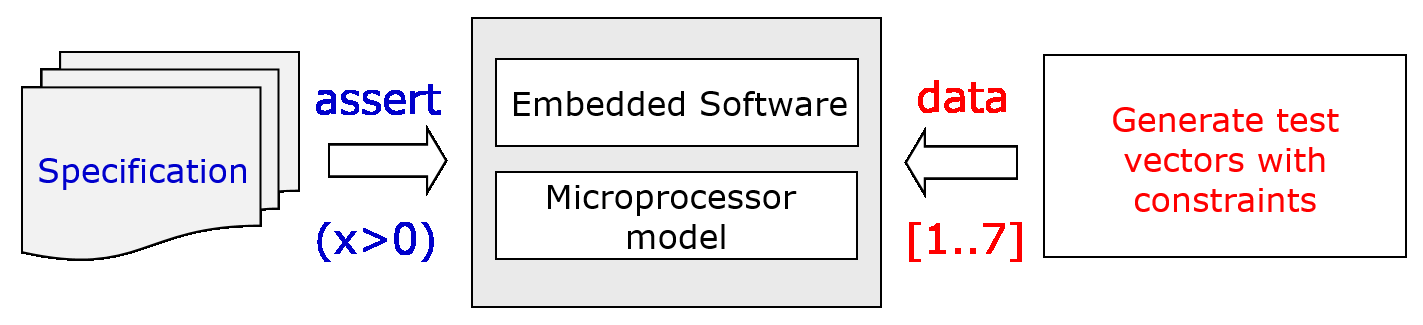
\includegraphics[scale=0.35]{figure2.eps}
	\caption{Verification methodologies for embedded systems.}
	\label{verification-methodologies}
\end{figure}


In particular, the main challenges regarding the verification of embedded systems lie on improving coverage, where more system functions are verified, reducing verification time, {\it i.e.}, pruning the state-space exploration during verification, and incorporating system models, which allow specific checks regarding system behavior and not only code correctness; additionally, embedded system verification raises additional challenges, such as 
%
\begin{enumerate}
	\item time and energy constraints;
	\item handling of concurrent software;
	\item platform restrictions; and
	\item legacy designs.%, which are usually developed with low-level languages.
\end{enumerate}

Indeed, the first two aspects are of extreme relevance in micro-grids and cyber-physical systems, in order to ensure reliability, which is a key issue for (smart) cities, industries, and consumers, and the third one is essential in systems that implement device models, such as digital filters and controllers, which present a behavior that is highly dependent on signal inputs and outputs and whose deployment may be heavily affected by hardware restrictions. The fourth aspect is inherent to a large number of embedded systems from  telecommunications, control systems, and medical devices.

%In summary, the main challenge when verifying embedded systems lies on improving coverage, where more system's functions are verified, and reducing verification time, {\it i.e.}, pruning the state-space exploration during verification. These aspects are of extreme relevance in micro-grids to ensure reliability, which is a key issue for (smart) cities and consumers.

%--------------------------------------
\section{Research Problem (RP)}
%--------------------------------------

This position paper tackles four major problems in computer-aided verification for embedded systems, which are (partially) open in present research.

\textbf{(RP1)} provide suitable encoding into the Satisfiability Modulo Theories (SMT) \cite{BarrettSST09}, which may extend the background theories typically supported by SMT solvers, with the goal of reasoning accurately and effectively about realistic embedded programs.

\textbf{(RP2)} exploit SMT techniques to leverage bounded model checking of multi-threaded software, in order to mitigate the state-explosion problem due to thread interleaving.
	
\textbf{(RP3)} prove correctness and timeliness of embedded systems, by taking into account stringent constraints imposed by hardware.
	
\textbf{(RP4)} incorporate knowledge about system purpose and associated features, which aims to detect system-level and behavior failures.

Section~\ref{achievements} outlines contributions toward these research problems.

%--------------------------------------
\section{Achievements}
\label{achievements}
%--------------------------------------

\textbf{(RP1)} Cordeiro, Fischer, and Marques-Silva proposed the first SMT-based BMC for full C programs, called Efficient SMT-Based Context-Bounded Model Checker (ESBMC)~\cite{Cordeiro12}, which was later extended to support C++98 programs~\cite{ECBS13}, CUDA programs~\cite{Pereira15}, and Qt-based consumer electronics applications~\cite{Sousa15}. This approach was also able to find undiscovered bugs related to arithmetic overflow, buffer overflow, and invalid pointer, in standard benchmarks, which were later confirmed by the benchmarks' creators ({\it e.g.}, NOKIA, NEC, NXP, and VERISEC)~\cite{CordeiroF11,Cordeiro12}. Other SMT-based BMC approaches have also been proposed and implemented~\cite{MerzFS12}, but the coverage and verification time of all existing ones are still limited to specific classes of programs, especially for those that contain intensive floating-point arithmetic and dynamic memory allocation~\cite{Beyer14,BeyerSVCOMP15}. One possible research direction is to bridge the gap between BMC tools and SMT solvers to propose theories and develop more efficient decision procedures, in order to handle specific classes of programs.

\textbf{(RP2)} The SMT-based BMC approach proposed by Cordeiro, Fischer, and Marques-Silva was further developed to verify correct lock acquisition ordering and the absence of deadlocks, data races, and atomicity violations in multi-threaded software based on POSIX and CUDA libraries~\cite{CordeiroF11,Pereira15}, considering monotonic partial-order reduction~\cite{KahlonWG09} and state-hashing techniques, in order to prune the state-space exploration~\cite{morse15}. Recent advances for verifying multi-threaded C programs have been proposed to speed up the verification time, which significantly prune the state-space exploration~\cite{Inverso14,civl15}. However, the class of concurrent programs ({\it e.g.}, CUDA, OpenCL, and MPI) that can be verified is still very limited. One possible research direction is to further extend BMC of multi-threaded C programs via Lazy Sequentialization~\cite{Inverso14}, in order to analyze unsatisfiability cores with the goal to remove redundant behaviour or to analyze interpolants to prove non-interference of context switches.

\textbf{(RP3)} Novel approaches to model check embedded software using \textit{k}-induction and invariants were proposed and evaluated in the literature, which demonstrate its effectiveness in some real-life embedded-systems applications~\cite{Gadelha15,Brain15,Rocha15}. However, the main challenge still remains open, {\it i.e.}, to compute and strengthen loop invariants to prove program correctness and timeliness in a more efficient and effective way, in order to be competitive with other model-checking approaches. In particular, invariant-generation algorithms have substantially evolved over the last years to discover inductive invariants of programs~\cite{pips:2013,Henry:2012} or to continuously refine them during verification~\cite{Beyer15}. However, there is still a lack of studies for exploiting the combination of different invariant-generation algorithms ({\it e.g.}, interval analysis, linear inequalities, polynomial equalities and inequalities) and how to strengthen them during verification, in order to ensure system robustness w.r.t. implementation aspects.

\textbf{(RP4)} State-of-the-art SMT-based context-BMC approaches were extended to verify overflow, limit cycle, time constraints, stability, and minimum phase, in digital systems; in particular, digital filters and controllers~\cite{dsv_spin2015,esbmc_controller,esbmc_filter}, and to specify system-level properties of those systems using linear-time temporal logic~\cite{JMorse15}. In particular, a specific UAV application was tackled, with the goal to verify its attitude controllers~\cite{Bessa16}. In general, however, there is still a lack of studies to verify system-level properties related to embedded systems; emphasis should be given to micro-grids~\cite{xu15} and cyber-physical systems~\cite{leeCPS2}, which require high-dependability requirements for computation, control, and communication. Additionally, the application of automated fault detection, localization, and correction techniques to digital systems represents an important research direction to make BMC tools useful for embedded systems engineers~\cite{Alves15}.

Lastly, yet importantly, BMC tools like CBMC~\cite{Clarke04}, ESBMC~\cite{MorseCNF13,MorseRCN014}, and LLBMC~\cite{MerzFS12} represent the most prominent ones for verifying C programs, as observed in the Intl. Competition on Software Verification~\cite{Beyer14,BeyerSVCOMP15}, where verifiable (correctness and violation) witnesses are of extreme importance for evaluating software verifiers~\cite{BeyerW15,RochaIFM12}.


%Finally, DSVerifier has already been used for verifying digital filters and controllers, which even include UAV applications. 


%--------------------------------------
\section{Conclusions}
\label{conclusions}
%--------------------------------------

This paper presented the main challenges related to the verification of design correctness in embedded systems. In particular, it emphasizes that stringent constraints imposed by the underlying hardware ({\it e.g.}, real-time, memory allocation, interrupts, and concurrency), along with system behavior models, must be considered during verification. Additionally, there is little evidence that model checking embedded software using \textit{k}-induction (and invariants), which
extends BMC-based approaches from falsification to verification, can be applied to formally verify correctness and timeliness of embedded systems. 

Given that software complexity has significantly increased in embedded products, there are still some (recent) advances to stress and exhaustively cover the system state space, in order to verify low-level properties that have to meet the application's deadline, access memory regions, handle concurrency, and control hardware registers. Besides, there is a trend towards incorporating knowledge about the system to be verified, which may take software verification one step further, where not only code correctness will be addressed, but also full system reliability. 

As future work, the main goal of this research is to extend BMC as a design and verification tool for achieving correct-by-construction embedded system implementations. Special attention will be given to cyber-physical systems and modern micro-grids, considering small-scale versions of a distributed system, so that reliability and other system-level properties ({\it e.g.}, carbon emission reduction in smart cities) are amenable to automated verification, probably through behavior models.



% conference papers do not normally have an appendix


% use section* for acknowledgment
\section*{Acknowledgment}

%The authors would like to thank...
The authors thank M. Dangl for reviewing a draft version of this paper.~This research was supported by CNPq $475647$/$2013$-$0$ grant.



\begin{thebibliography}{1}

%1
\bibitem{Kopetz11}
H.~Kopetz:
\newblock {\em Real-Time Systems - Design Principles for Distributed Embedded Applications}.
\newblock Real-Time Systems Series, Springer, ISBN 978-1-4419-8236-0, pp. 1--376, 2011.

%2
\bibitem{xu15}
Xua X., Jiaa H., Wanga D., Yub D., Chiangc H.:
\newblock {\em Hierarchical energy management system for multi-source multi-product microgrids}
\newblock In: Renewable Energy, v. 78, pp. 621--630, 2015.

%3
\bibitem{leeCPS}
Lee E.:
\newblock {\em Cyber-physical Systems: Design Challenges.} 
\newblock In: International Symposium on Object Oriented Real-Time Distributed Computing, pp. 363--369, 2008.

%4
\bibitem{leeCPS2}
Lee E.:
\newblock {\em The Past, Present and Future of Cyber-Physical Systems: A Focus on Models}. 
\newblock In: Sensors 15(3): pp. 4837--4869, 2015.

%5
\bibitem{groza2015formal}
Groza A., Letia I., Goron A., Zaporojan S.: 
\newblock {\em A formal approach for identifying assurance deficits in unmanned aerial vehicle software}
\newblock In: Progress in Systems Engineering, Springer, pp. 233--239, 2015.

%6
\bibitem{Cordeiro09}
Cordeiro L., Fischer B., Chen H., Marques-Silva J.:
\newblock {\em Semiformal Verification of Embedded Software in Medical Devices Considering Stringent Hardware Constraints.} 
\newblock In: International Conference on Embedded Software and Systems, pp. 396--403, 2009.

%7
\bibitem{munir}
Munir  S., Stankovic J. A., Liang C.-J. M., Lin S.:
\newblock {\em Cyber Physical System Challenges for Human-in-the-Loop Control}. 
\newblock In: 8th International Workshop on Feedback Computing, pp. 1--4, 2013.

%8
\bibitem{Kroening15}
Kroening D., Liang L., Melham T., Schrammel P., Tautschnig M.:
\newblock {\em Effective Verification of Low-Level Software with Nested Interrupts}. 
\newblock In: Design, Automation and Test in Europe, pp. 229--234, 2015.

%9
\bibitem{Biere99}
Biere A., Cimatti A., Clarke E., Zhu Y.:
\newblock {\em Symbolic Model Checking without BDDs}. 
\newblock In: Tools and Algorithms for Construction and Analysis of Systems, LNCS 1579, pp. 193--207, 1999.

%10
\bibitem{handbook09}
Biere A., Heule M., van Maaren H., Walsh T., eds.:
\newblock {\em Handbook of Satisfiability}.
\newblock Volume 185 of Frontiers in Artificial Intelligence and Applications., {IOS} Press, 2009.

%11
\bibitem{BarrettSST09}
Barrett C., Sebastiani R., Seshia S.A., Tinelli C.:
\newblock {\em Satisfiability Modulo Theories}. 
\newblock In: Volume 185 of Frontiers in Artificial Intelligence and Applications. IOS Press, pp. 825--885, 2009.

%12
\bibitem{Armando06}
Armando A., Mantovani J., Platania L.:
\newblock {\em Bounded Model Checking of Software Using SMT Solvers Instead of SAT Solvers}. 
\newblock In: {SPIN} Workshop on Model Checking Software, LNCS 3925, pp. 146-162, 2006.

%13
\bibitem{Clarke04}
Clarke E., Kroening D., Lerda F.:
\newblock {\em A Tool for Checking {ANSI-C} Programs.}
\newblock In: Tools and Algorithms for the Construction and Analysis of Systems. LNCS 2988, Springer Berlin Heidelberg, pp. 168--176, 2004.

%14
\bibitem{MerzFS12}
Merz F., Falke S., Sinz C.:
\newblock {\em {LLBMC}: Bounded Model Checking of {C} and {C++} Programs using a Compiler {IR}.}
\newblock In: International Conference on Verified Software: Theories, Tools, Experiments. LNCS 7152, pp. 146--161, 2012.

%15
\bibitem{CordeiroF11}
Cordeiro L., Fischer B.:
\newblock {\em Verifying Multi-threaded Software using {SMT}-based Context-Bounded Model Checking.}
\newblock In: International Conference on Software Engineering. pp. 331--340, 2011.

%16
\bibitem{Ivancic05}
Ivanicic F., Shlyakhter I., Gupta A., Ganai, M.K.:
\newblock {\em Model Checking {C} Programs using {F-Soft}.}
\newblock In: International Conference on Computer Design: VLSI in Computers and Processors, pp. 297--308, 2005.

%17
\bibitem{Cordeiro12}
Cordeiro L., Fischer B., Marques{-}Silva J.:
\newblock {\em {SMT}-based Bounded Model Checking for Embedded {ANSI-C} Software}.
\newblock {IEEE} Trans. Software Eng. \textbf{38}(4), pp. 957--974, 2012.

%18
\bibitem{EenS03}
E{\'{e}}n, N., S{\"{o}}rensson, N.:
\newblock {\em Temporal Induction by Incremental {SAT} Solving.}
\newblock Electronic Notes in Theoretical Computer Science \textbf{89}(4), pp. 543 -- 560, 2003.

%19
\bibitem{Sheera00}
Sheeran M., Singh S., St{\aa}lmarck G.:
\newblock {\em Checking Safety Properties using Induction and a {SAT}-solver.}
\newblock In: International Conference on Formal Methods in Computer-Aided Design. Springer-Verlag, pp. 108--125, 2000.

%20
\bibitem{Bradley07}
Bradley A., Manna Z.:
\newblock {\em The calculus of computation - decision procedures with applications to verification}. 
\newblock In: Springer, pp. I-XV, pp. 1--366, 2007.

%21
\bibitem{pips:2013}
ParisTech M.:
\newblock {\em PIPS: Automatic Parallelizer and Code Transformation Framework.} 
\newblock Accessed 21 February 2016

%22
\bibitem{Henry:2012}
Henry J., Monniaux D., Moy M.: 
\newblock {\em PAGAI: A Path Sensitive Static Analyser.} 
\newblock In: Electronic Notes in Theoretical Computer Science, pp. 15--25, 2012.

%23
\bibitem{Gadelha15}
Gadelha M., Ismail H., Cordeiro L.:
\newblock {\em Handling Loops in Bounded Model Checking of C Programs via \textit{k}-Induction.}
\newblock In: International Journal on Software Tools for Technology Transfer (to appear), 2015.
\newblock http://dx.doi.org/10.1007/s10009-015-0407-9

%24
\bibitem{Beyer15}
Beyer D., Dangl M., Wendler P.:
\newblock {\em Boosting \textit{k}-Induction with Continuously-Refined Invariants.}
\newblock In: International Conference on Computer-Aided Verification, LNCS 9206, pp. 622--640, 2015.

%25
\bibitem{Brain15}
Brain M., Joshi S., Kroening D., Schrammel P.:
\newblock {\em Safety Verification and Refutation by k-Invariants and \textit{k}-Induction.}
\newblock In: International Symposium on Static Analysis, LNCS 9291, pp. 145--161, 2015.

%26
\bibitem{Rocha15}
Rocha H., Ismail H., Cordeiro L., Barreto R.:
\newblock {\em Model Checking Embedded C Software using \textit{k}-Induction and Invariants.}
\newblock V Brazilian Symposium on Computing Systems Engineering, pp. 90--95, 2015.

%27
\bibitem{Donaldson10}
Donaldson A., Kroening D., R{\"{u}}mmer P.:
\newblock {\em {SCRATCH}: A Tool for Automatic Analysis of {DMA} Races.}
\newblock In: ACM Symposium on Principles and Practice of Parallel Programming. ACM, pp. 311--312, 2011.

%28
\bibitem{Kinductor}
Donaldson A., Haller L., Kroening D., R{\"{u}}mmer, P.:
\newblock {\em Software Verification using \textit{k}-Induction.}
\newblock In: International Conference on Static Analysis. LNCS 6887, pp. 351--368, 2011.

%29
\bibitem{GrosseLD09}
Gro{\ss}e D., Le H., Drechsler R.:
\newblock {\em Induction-based Formal Verification of {SystemC TLM} Designs.}
\newblock In: International Workshop on Microprocessor Test and Verification, pp. 101--106, 2009.

%30
\bibitem{Behrend15}
Behrend J., Lettnin D., Gruenhage A., Ruf J., Kropf T., Rosenstiel W.:
\newblock {\em Scalable and Optimized Hybrid Verification of Embedded Software}. 
\newblock In: J. Electronic Testing 31(2): pp. 151--166, 2015.

%31
\bibitem{dsv_spin2015}
Ismail H., Bessa I., Cordeiro L., Lima Filho E., Chaves Filho J.:
\newblock {\em DSVerifier: A Bounded Model Checking Tool for Digital Systems}. 
\newblock In: International SPIN Symposium on Model Checking of Software, LNCS 9232, pp. 126--131, 2015.

%32
\bibitem{Lettnin09}
Lettnin D., Nalla P. K., Behrend J., Ruf J., Gerlach J., Kropf T., Rosenstiel W., Sch{\"o}nknecht V., Reitemeyer S.:
\newblock {\em Semiformal Verification of Temporal Properties in Automotive Hardware Dependent Software}. 
\newblock In: Design, Automation and Test in Europe, pp. 1214--1217, 2009.

%33
\bibitem{Beyer14}
D.~Beyer 
\newblock {Status report on software verification - (competition summary {SV-COMP})}. 
\newblock In: Tools and Algorithms for the Construction and Analysis of Systems, LNCS 8413, pp. 373--388, 2014.
 
%34
\bibitem{BeyerSVCOMP15}
D.~Beyer:
\newblock {\em Software Verification and Verifiable Witnesses - (Report on SV-COMP 2015).} 
\newblock In: Tools and Algorithms for the Construction and Analysis of Systems, LNCS 9035, pp. 401-416, 2015.

%35
\bibitem{Inverso14}
Inverso O., Tomasco E., Fischer B., La Torre S., Parlato G.:
\newblock {\em Bounded Model Checking of Multi-threaded C Programs via Lazy Sequentialization.}
\newblock In: International Conference on Computer-Aided Verification, LNCS 8559, pp. 585-602, 2014.

%36
\bibitem{ECBS13}
Ramalho M., Lopes M., Sousa F., Marques H., Cordeiro L., Fischer B.:
\newblock {\em {SMT-Based Bounded Model Checking of C++ Programs} }.
\newblock In: International Conference on Engineering of Computer-Based Systems, pp. 147--156, 2013.

%37
\bibitem{Pereira15}
Pereira P.  Albuquerque H., Marques H., Silva I., Carvalho C., Santos V., Ferreira R., Cordeiro L.: 
\newblock {\em Verifying CUDA Programs using SMT-Based Context-Bounded Model Checking.} 
\newblock In: ACM Symposium on Applied Computing, Software Verification and Testing Track, pp. 1648-1653, 2016. 

%38
\bibitem{Sousa15}
Sousa F., Cordeiro L., Lima Filho E.: 
\newblock {\em { Bounded Model Checking of C++ Programs Based on the Qt Framework.}} 
\newblock In: Global Conference on Consumer Electronics, pp. 179--180, 2015.

%39
\bibitem{morse15}
J.~Morse.
\newblock {\em {Expressive and Efficient Bounded Model Checking of Concurrent Software}}.
\newblock {University of Southampton, PhD Thesis}, 2015.

%40
\bibitem{civl15}
Zheng M, Rogers M, Luo Z, Dwyer M, Siegel S.
\newblock {\em{{CIVL}: Formal Verification of Parallel Programs}}.
\newblock In: International Conference on Automated Software Engineering, pp. 830--835, 2015.

%41
\bibitem{esbmc_controller}
Bessa I., Abreu R., Cordeiro L., Filho J.:
\newblock {\em {SMT-Based Bounded Model Checking of Fixed-Point Digital Controllers)}.}
\newblock In: Annual Conference of the Industrial Electronics Society, pp. 295--301, 2014.

%42
\bibitem{esbmc_filter}
Abreu R., Cordeiro L., Filho E.:
\newblock {\em {Verifying Fixed-Point Digital Filters using SMT-Based Bounded Model Checking}.}
\newblock In: XXXI Brazilian Symposium on Telecommunications, 2013.
\newblock http://dx.doi.org/10.14209/sbrt.2013.57

%43
\bibitem{JMorse15}
Morse J., Cordeiro L., Nicole D., Fischer B.:
\newblock {\em {Model Checking LTL Properties over ANSI-C Programs with Bounded Traces.}} 
\newblock In: Software and System Modeling 14(1): pp. 65--81, 2015.

%44
\bibitem{Bessa16}
Bessa I., Ismail H., Cordeiro L., Chaves Filho J.:
\newblock {\em { Verification of Fixed-Point Digital Controllers Using Direct and Delta Forms Realizations.}} 
\newblock In: Design Automation for Embedded Systems (to appear), 2016.

%45
\bibitem{MorseCNF13}
Morse J., Cordeiro L., Nicole D., Fischer B.:
\newblock {\em Handling unbounded loops with {ESBMC} 1.20.}
\newblock In: Tools and Algorithms for the Construction and Analysis of
  Systems. LNCS 7795, Springer Berlin Heidelberg, pp. 619--622, 2013.

%46
\bibitem{MorseRCN014}
Morse J., Ramalho M., Cordeiro L., Nicole D., Fischer B.:
\newblock {\em {ESBMC} 1.22.}
\newblock In: Tools and Algorithms for the Construction and Analysis of
  Systems. LNCS 8413, Springer Berlin Heidelberg, pp. 405--407, 2014.

%47
\bibitem{KahlonWG09}
Kahlon V., Wang C., Gupta A.:
\newblock {\em{Monotonic Partial Order Reduction: An Optimal Symbolic Partial Order Reduction Technique}}.
\newblock In: International Conference on Computer-Aided Verification, LNCS 5643, pp. 398--413, 2009.

%48
\bibitem{Alves15}
Alves E. , Cordeiro L., Lima Filho E.:
\newblock {\em{ Fault Localization in Multi-Threaded C Programs using Bounded Model Checking}}. 
\newblock In: Brazilian Symposium on Computing Systems Engineering, pp. 96-101, 2015.

%49
\bibitem{BeyerW15}
Beyer D., Dangl M., Dietsch D., Heizmann M., Stahlbauer A.:
\newblock {\em{ Witness validation and stepwise testification across software verifiers}}. 
\newblock In: ESEC/SIGSOFT Foundations of Software Engineering, pp. 721--733, 2015.

%50
\bibitem{RochaIFM12}
Rocha H., Barreto R., Cordeiro L., Dias Neto A.:
\newblock {\em{ Understanding Programming Bugs in ANSI-C Software Using Bounded Model Checking Counter-Examples}}. 
\newblock In: International Conference on Integrated Formal Methods, LNCS 7321, pp. 128-142, 2012.

\end{thebibliography}




% that's all folks
\end{document}


